
% \documentclass{sig-alternate-05-2015}
\documentclass[9pt, numbers]{sigplanconf}


% The following \documentclass options may be useful:

% preprint      Remove this option only once the paper is in final form.
% 10pt          To set in 10-point type instead of 9-point.
% 11pt          To set in 11-point type instead of 9-point.
% authoryear    To obtain author/year citation style instead of numeric.

\usepackage{amsmath}
% \usepackage[numbers,sort]{natbib}
\usepackage{url}
%\usepackage{subfigure}
\usepackage{listings}
%\usepackage{subfig}
\usepackage{eqnarray}

\usepackage{graphicx}
\usepackage{algorithm}
%\usepackage{algorithmicx}
%\usepackage{algorithmic}
\usepackage{algpseudocode}
\usepackage{mathtools}
\usepackage{caption}
\usepackage{subcaption}
\usepackage{diagbox}

\usepackage{color}
\newcommand{\jli}{\textcolor[rgb]{1,0,0}{JL: }\textcolor[rgb]{1,0,0}}
\definecolor{mygray}{gray}{0.4}
\renewcommand{\algorithmiccomment}[1]{ \hfill \(\triangleright\) {\color{mygray}{#1}} }

\graphicspath{{./Figures/}}

\algdef{SE}[DOWHILE]{Do}{doWhile}{\algorithmicdo}[1]{\algorithmicwhile\ #1}
\algnewcommand{\LeftComment}[1]{\Statex \(\triangleright\) #1}
\algnewcommand{\LineComment}[1]{\State \(\triangleright\) {\color{mygray}{#1}}}

%\makeatletter
%\algnewcommand{\LineComment}[1]{\Statex \hskip\ALG@thistlm \(\triangleright\) #1}
%\makeatother


% distance between floats on the top or the bottom and the text;
% \setlength{\textfloatsep}{0pt} % plus 0.5pt minus 0.5pt} 
% % distance between two floats;
% \setlength{\floatsep}{0pt}
% % distance between floats inserted inside the page text (using h) and the text proper.
% \setlength{\intextsep}{0pt} 
% %plus 0.5pt minus 0.5pt % between figure and caption
% \setlength{\abovecaptionskip}{1pt} 
% %%
% \setlength{\abovedisplayskip}{0pt}
% \setlength\belowdisplayskip{0pt}
% \setlength\abovedisplayshortskip{0pt}
% \setlength\belowdisplayshortskip{0pt}


\begin{document}

\conferenceinfo{PPoPP~'17}{Feb. 4--8, 2017, Austin, Texas, USA.} 
\copyrightyear{2017} 
\copyrightdata{978-1-4503-4493-7/17/02} 
%\doi{nnnnnnn.nnnnnnn} 
%\setcopyright{acmcopyright}

%\conferenceinfo{XXXX 'XX}{Month d--d, 20yy, City, ST, Country}
%\acmPrice{\$15.00}

% Uncomment one of the following two, if you are not going for the
% traditional copyright transfer agreement.

%\exclusivelicense                % ACM gets exclusive license to publish,
                                  % you retain copyright

%\permissiontopublish             % ACM gets nonexclusive license to publish
                                  % (paid open-access papers,
                                  % short abstracts)

%\titlebanner{}        % These are ignored unless
%\preprintfooter{}   % 'preprint' option specified.

\title{Understanding GPU Microarchitecture to Achieve Bare-Metal Performance Tuning}
\subtitle{}


\authorinfo{Name1}
           {Affiliation1}
           {Email1}
\authorinfo{Name2\and Name3}
           {Affiliation2/3}
           {Email2/3}

\maketitle

\begin{abstract}
In this paper, we present a methodology to demystify GPU microarchitectural features and demonstrate the performance tuning experience for compute-intensive kernels. The methodology relies on a reverse engineering approach to cracking the GPU ISA instruction encodings to build a GPU assembler.
An assembly microbenchmark suite correlates microarchitectural features with their performance factors and uncovers float instruction dual issue, memory load width, register bank, and other microarchitectural features. We use SGEMM as a running example throughout this paper to show how to achieve bare-metal performance tuning. The performance boost is achieved by tuning {\tt FFMA} throughput to the hardware peak by activating dual issue, eliminating register bank conflicts, adding non-{\tt FFMA} instructions with little penalty, and choosing proper width of global/shared load instructions.
On NVIDIA Kepler K20m, we develop a faster SGEMM with $3104$Gflop/s performance and $88\%$ efficiency, which is $15\%$ higher than cuBLAS7.0 .
Applying these optimizations on convolutional networks, the optimized implementations gains $39\%$-$62\%$ performance improvement compared to cuDNN4.0.
The toolchain is an attempt to automatically crack different GPU ISA encodings and build a complete assembler adaptively, to explore more performance for applications on GPUs.
% , and instruction scheduling.
% The optimized SGEMM achieves $3104$ Gflop/s and its efficiency is $88\%$, which is $15\%$ higher than cuBLAS7.0 on NVIDIA Kepler K20m.
% We believe that our SGEMM optimization can serve as an example of how to optimize other float computation-intensive algorithm on GPU.
\end{abstract}


%\category{CR-number}{subcategory}{third-level}

% general terms are not compulsory anymore,
% you may leave them out
%\terms
%term1, term2

\keywords
SGEMM, Assembler, GPU, Performance
\section{Introduction}
Single-precision General Matrix Multiply (SGEMM), as one 
of the basic routines in a BLAS library~\cite{blas,intel2007intel,amd2014}, performs a multiplication of two single-precision matrices. 
It has been extensively used in many scientific and engineering 
computing applications. 
Recently, increasing efforts have been made to tune the performance of SGEMM, because of its critical performance effect on deep learning applications~\cite{chetlur2014cudnn,nervana_sgemm_wiki}.
% as it is a performance critical kernel in
%In convolutional neural network (CNN), the most expensive fully-connected and convolution layers can be implemented using
%SGEMM~\cite{chetlur2014cudnn}.
%In the presence of statistical approximation and estimation errors, the computation of deep learning is not sensitive to
%high precision~\cite{Gupta}. In this work, we focus on SGEMM optimization.

As GPUs provide higher peak floating-point performance and memory bandwidth than CPUs contemporarily, researchers tend to adopt GPUs to accelerate compute-intensive programs. 
%In fact, SGEMM's performance highly relies on low-level microarchitecture features. 
Hardware vendors provide BLAS libraries specifically tuned for their own processors, such as Intel MKL~\cite{intel2007intel} and AMD ACML~\cite{amd2014} for multicore x86 CPUs and NVIDIA cuBLAS~\cite{intel2007intel} and AMD CLMath~\cite{clmath} for GPUs. 
However, we always witness performance improvement from third-party implementations over these vendor libraries. 
For example, OpenBLAS~\cite{xianyi2012openblas}, based on its hand-tuned assembly codes, achieves the highest performance in most cases on a multicore x86\jli{correct?} CPU.
Although an OpenBLAS-like library is absent from GPUs, several % ongoing 
efforts~\cite{tan,lai,nervana_sgemm_wiki,
chien, volkov} have achieved better performance than cuBLAS for (S/D)GEMM by tuning assembly codes on NVIDIA GPUs. 
However, % accomplish the microarchitecture based performance tuning on every GPU generation
the disperse work leaves two issues to be addressed for diligently tuning the SGEMM performance on the microarchitecture of every GPU generation.
\begin{itemize}
\item {\em A lack of a toolchain to identify GPU microarchitecture features and guide performance tuning.}
  Unlike the general-purpose CPU community where a series of toolchains are available to tune performance in a bare-metal
  way, only the abstract CUDA model is encouraged in the GPU community. 
  NVIDIA engineers hand tune their supported % cuBLAS routines and other vendor
  libraries in GPU assembly language, this leaves other unsupported algorithms hard to be diligently optimized.
  %The main reason is the significant changes of GPU architecture
  %among generations. For example, graphic features, register bank distribution, and floating-point instructions dual
  %issue of the recent ISAs are totally different from the previous generations~\cite{fermi}. 
  Fortunately, researchers have made some initial progress on performance tuning tools, including benchmarking~\cite{mei, volkov, wong} and designing assemblers~\cite{asfermi,bernstein2012usable,decuda,maxas} on some particular GPU architectures\jli{further check}.
% to pursue extreme performance. 
In this paper, we develop a methodology to systematically identify 
microarchitecture by automatically decoding instruction formats, generating ISA-compatible binaries, and benchmarking.
\item {\em A lack of comprehensive understanding of the SGEMM performance behavior in terms of the low-level GPU microarchitecture.} 
Most SGEMM analyses are circumscribed at CUDA or PTX level due to the short of GPU bare-metal tools. 
Therefore, these studies cannot directly diagnose compiler deficiency or hardware 
defects. 
By observing the disassembled codes of CUDA SGEMM, we find that the CUDA compiler (NVCC) generated control codes are deficient in exploiting FP32 Fused Multiply Add ({\tt FFMA}) dual issue (details in section~\ref{sec:ffma-dual}). 
This indicates the binary codes cannot completely utilize GPU cores but leave some of them idle most of the time. 
% completely utilize all cores in a streaming processor (SM), 
A side effect of this compiler deficiency leads to a bias estimation of the performance bound. 
This paper presents a thorough performance analysis which goes through the whole architecture hierarchy, including instruction 
throughput, register allocation, and shared/global memory transfers. 
The identified microarchitecture features help us build robust performance models of SGEMM and other programs.
\end{itemize}

In this paper, we propose a GPU ISA encoding solver to automatically crack GPU ISA encodings from GPU disassembly codes,
then we build a GPU assembler to generate binaries from hand-optimized assembly codes.\jli{further check}%CUDA binary files. 
Taking the advantage of the compatible grammar of CUDA {\tt cuobjdump}~\cite{cubin2015util} with NVCC~\cite{nvcc}, we use NVCC to compile CUDA codes to a {\em cubin} file and 
then disassemble it to assembly codes. 
This approach allows users to optimize any code segment based on the generated assembly codes instead of coding from scratch. 
With this assembler, a microbenchmark suite is designed to 
demystify plenty of GPU microarchitecture features such as instruction issue, warp scheduling, and register bank distribution, which help understand and optimize the performance of a computational program. 
We apply optimization methods corresponding to GPU microarchitecture features to improve SGEMM performance incrementally. 
More specifically, we make the following contributions:

\begin{itemize}
\item We propose a GPU ISA encoding solver to automatically crack ISA encodings
     of diverse GPU microarchitectures from disassembly codes.
%instruction encoding of GPU architecture.
A Kepler GPU assembler is developed to directly tune the assembly codes generated by CUDA compiler.
\item We design a microbenchmark suite to explore undocumented
microarchitecture features of NVIDIA GPUs, such as control codes regulating
{\tt FFMA} instruction dual issue and register bank indices influence
instruction throughput, which are necessary to understand and tune GPU
programs.
\item We implement the SGEMM routine on a NVIDIA Kepler GPU by applying the demystified microarchitecture-level optimizations. 
The optimized SGEMM achieves up to 88\% of the machine's peak floating-point performance, which is 15\% higher than the state-of-the-art SGEMM in cuBLAS.
\end{itemize}

%Albeit Kepler is not the latest generation GPU, the {\tt FFMA} dual-issue feature will not be
%outdated. During our exploring of the method to fully exploit the arithmetic
%dual-issue feature of Kepler, we find that NVCC can not generate dual issue code efficiently even for computation
%intensive SGEMM which prevents dual issue feature further development in the succeeding GPUs. The Dual-issue feature would return in future
%GPU design when scalability of thread level parallelism and frequency of GPU are too hard to improve.
Although this work demonstrates the effectiveness of our methodology on a NVIDIA Kepler GPU, the methodology is general-purpose for 
other NVIDIA GPU architectures under minor adjustments of instruction solver and benchmarking. 
% To the best of our knowledge, it is the first time to provide a detailed description of how to crack the instruction encoding for NVIDIA GPUs automatically.
To the best of our knowledge, it is the first time to thoroughly describe the automatic cracking of the instruction encodings of NVIDIA GPUs
\footnote{\scriptsize{Code:https://github.com/PAA-NCIC/PPoPP2017\_artifact}}. 
The experience of 
exploring bare-metal optimizations is helpful\jli{``valuable'' may be too much} to compiler development and performance tuning.

The rest of this paper is organized as follows. Section~\ref{sec:background} introduces 
a general blocking SGEMM algorithm and the CUDA binary utilities.
Section~\ref{sec:assembler} presents the instruction solver algorithms and
microbenchmarking 
insights. Section~\ref{sec:optimization} applies a series of microarchitectural optimizations to SGEMM. We report 
experimental results in section~\ref{sec:experiment}.
Section~\ref{sec:generality} discusses the generality and portability of our methodology for different GPUs and diverse algorithms.
Section~\ref{sec:related} summarizes the related work. Finally, 
section~\ref{sec:conclusion} concludes this work. 

\section{Background}
\label{sec:background}

This section first highlights tunable factors that determine SGEMM performance on the GPU architecture, then introduces some CUDA binary utilities related to SGEMM optimization at assembly level for self-containment. 
% Since we seek to optimize SGEMM at assembly-level, this section introduces some CUDA binary utilities used in our work. 


\subsection{Performance Factors of SGEMM}
\label{sec:sgemm}
%It's well-known that the primary factors of SGEMM performance are the blocking parameters for exploiting data reuse 
%through memory hierarchy. On GPUs, we should consider both shared memory blocking and register blocking. For the 
%purpose of completeness, we describe a blocking algorithm which is similar to that in other 
%literature~\cite{magma,nervana_sgemm_wiki,lai,tan}.
The state of art implementation of SGEMM on GPU~\cite{magma,nervana_sgemm_wiki,lai,tan} uses two level blocking:
shared memory blocking and register blocking to exploit data reuse through memory hierarchy.
%SGEMM is to evaluate the product $C = C + AB$, where $A$, $B$ and $C$ are $m\times k$, $k\times n$ and $m\times n$
The GEMM routines compute a scalar-matrix-matrix product and add the result to
a scalar-matrix product, with general matrices. The operation is defined as $C
= beta*C + alpha*AB$, where $A$, $B$ and $C$ are $m\times k$, $k\times n$ and
$m\times n$ matrices respectively, while alpha and beta are float scalar constants respectively.

Algorithm~\ref{gemm} shows the skeleton of SGEMM blocking algorithm. Task partition is based on the result matrix $C$. 
Each thread block with $t_x*t_y$ threads is responsible to compute a $b_m*b_n$ submatrix in $C$, where $b_m, b_n$ are the 
number of rows and columns of the submatrix $A$ and $B$ respectively. We need to read a $b_m*b_k$ from $A$ and a $b_k*b_n$ sub-matrix from 
$B$ for each thread block, where $b_k$ is the unrolling factor. In this way, $A$, $B$ and $C$ are divided into $M*K$, $K*N$ and 
$M*N$ grids of $b_m*b_k$, $b_k*b_n$ and $b_m*b_n$ blocks, where $M=\Bigl\lfloor \frac{m+b_m-1}{b_m} \Bigr\rfloor$, 
$K=\Bigl\lfloor \frac{k+b_k-1}{b_k} \Bigr\rfloor$, $N=\Bigl\lfloor \frac{n+b_n-1}{b_n} \Bigr\rfloor$.

\begin{algorithm}
  \caption{SGEMM blocking algorithm. {\em smA} and {\em smB} are shared memory variables. {\em rA}, {\em rB} and {\em 
accum} are register variables. $r_x$ and $r_y$ are register blocking sizes}
  \label{gemm}
  \begin{algorithmic}[1]
	\LineComment {The size of a thread block: $t_x*t_y$}
	\LineComment {Registers: accum[$r_x*r_y$], rA[$2*r_x$], rB[$2*r_y$]}
	\State $smA[b_m][b_k] \gets$ a $b_m * b_k$ block of $A$
	\State $smB[b_k][b_n] \gets$ a $b_k * b_n$ block of $B$
	\Do
      \For {{$i \gets 1, b_k$}}
      %\Comment {\color {mygray} {Unrolling for loop}}
      \Comment {{Unrolling for loop}}
      \State {\color {black} {$rA[0...r_x]\gets$ a column of $smA$}}
	\State $rB[0...r_y]\gets$ a row of $smB$
	\State $accum[0...r_x][0...r_y]\gets accum[0...r_x][0...r_y]+rA[0...r_x]*rB[0...r_y]$
	\EndFor
	\State $smA[b_k][b_m]\gets$ a $b_m*b_k$ block of $A$
	\State $smB[b_k][b_n]\gets$ a $b_k*b_n$ block of $B$
	\State \textbf{sync}
	\doWhile {pointer in $B$ is not out of range}
	\State \textbf{merge} $accum[0...r_x][0...r_y]$ with a $b_m*b_n$ block of $C$.
  \end{algorithmic}
\end{algorithm}

The volume of float point computations inside the while loop of Algorithm~\ref{gemm} is $2\times r_x\times r_y \times b_k$ 
in operations, and Table~\ref{tab:dm} estimates data movement volume through registers, shared memory, and global 
memory for each thread inside the while loop.
These parameters demonstrate that SGEMM performance is affected by the hierarchical memory blocking and unrolling 
factors in the inner loops.
The tuning of these factors is conducted in two folds:memory bandwidth and latency. In fact, with the estimations in 
Table~\ref{tab:dm}, it is relatively easy to tune proper parameters to eliminate the bound of memory 
bandwidth~\cite{magma}~\cite{tan}. The difficulty lies in latency, which is closely related to specific 
microarchitectures such as instruction sequence and instruction type. However, the microarchitectural 
optimizations depend on the availability of an assembler and deep understanding of microarchitectural features.

\begin{table}[htbp]
    \caption{Data movement volume of each thread inside the while loop.} %\jled{this table is not referred in this paper.}}
\centering
\scalebox{1.0} {
\begin{tabular}{|c|c|}
\hline
    Data path& Volume(in words)\\
\hline
    global$\Rightarrow$register ({\tt LDG})& $\frac{r_x*\times r_y \times b_k}{b_m} + \frac{r_x\times r_y \times b_k}{b_n}$ \\
\hline
register$\Rightarrow$shared ({\tt STS})& $\frac{r_x*\times r_y \times b_k}{b_m} + \frac{r_x\times r_y \times b_k}{b_n}$ \\
\hline
shared$\Rightarrow$register ({\tt LDS})& $r_x\times b_k + r_y\times b_k$\\
\hline
%    arithemtic({\tt FFMA})& $r_x\times r_y \times b_k$\\
%\hline
\end{tabular}
}
\label{tab:dm}
\end{table}
\subsection{CUDA Binary Utilities}
\label{sec:cuda}
%NVIDIA does not release its GPU assembler to public, they release other tool-chains:ptxas, nvcc.
Though no official GPU assembler is public avaible, NVIDIA provides PTX assembly compiler {\tt PTXAS}, disassembly tools {\tt cuobjdump} and {\tt nvdisasm} which make it possible to build a GPU assembler by third-party.
For instance, both {\tt cuobjdump} and {\tt nvdisasm} disassemble {\em cubin} files to {\em sass} files, which are 
readable assembly codes for examining possible performance issues in GPU programs. For each instruction in the 
executable code sections, the tools list its address in hexadecimal, mnemonics in a string, and encoded number in 
hexadecimal. For example, an {\tt IADD} instruction might be printed as follows: \\\\
$/*0048*/~~~~IADD~~R0,~~R2,~~R0;~~/* 0x4800000000201c03 */$\\\\
Unfortunately, these tools do not enable us to modify the assembly codes directly for tuning performance. What we can 
do is to refine CUDA C codes after examining the read-only assembly codes iteratively. Therefore, an assembler is 
required to manipulate assembly codes. Although NVIDIA does not release its internal assembler and instruction encoding 
format, the disassembled code and the released pseudo assembly references~\cite{ptx2015isa}, provide us clues to crack 
instruction format (in Section~\ref{sec:assembler}).
%NVIDIA provides {\tt PTXAS} to compile PTX assembly to cubin.
%PTX is a low-level parallel thread execution virtual machine and instruction set architecture (ISA)~\cite{}.
%The goals for PTX include the following:
PTX defines a virtual machine and ISA for general purpose parallel thread execution.
%PTX programs are translated at install time to the target hardware instruction set. The
%PTX-to-GPU translator and driver enable NVIDIA GPUs to be used as programmable
%parallel computers. 
The goal of PTX is to provide a stable machine-independent
ISA that spans multiple GPU generations for compilers to target.
Since PTX assembly is machine-independent, it is a kind of pseudo-assembly. There are several disadvantages of it:
First, PTX assembly use pseudo-registers, you can not control register
allocation. Second, as Kepler and Maxwell GPU use control code to do warp
scheduling, but in PTX assembly no control code information.
By using {\tt PTXAS}, we could compile PTX code to Cubin, then use disassemble
tool {\tt cuobjdump} to generate the native assembly with control code. The disassembly is the input of GPU ISA solver.
%PTX exposes the GPU as a data-parallel computing device.
%We can only use CUDA/OpenCL and PTX on NVIDIA GPU, no assembly is supported publicly by NVIDIA company. 
%\jled{introduce instruction and some mentioned opcodes in this paper.}
%A CUDA binary file, also called {\em cubin}, is an ELF-formatted file generated by CUDA compiler ({\tt nvcc}). It can 
%be either embedded into a host executable file or generated separately by using the "{\em -cubin}" option of {\tt 
%nvcc}. To help developers understand {\em cubin} files, CUDA toolkit introduces binary tools and documents on ISAs from 
%GT200 to Maxwell architecture~\cite{gtx980}. These binary tools only provide very limited functionalities for users. 

\section{Demystify Microarchitecture Features}
\label{sec:assembler}
\subsection{Methodology}


We propose a methodology to demystify GPU microarchitectural features and correlate them with microbenchmark performance.
The workflow in Figure~\ref{fig:workflow} consists of three major components: a GPU ISA encoding solver, a GPU assembler, and the meticulous benchmarks.
The sample programs in Figure~\ref{fig:workflow} are synthetic PTX files which generate specific instructions as the input of the instruction solver.
Deliberate microbenchmarks are designed in assembly to figure out the correlation between microarchitecture and performance.
%We dissemble a binary library (such as cuBLAS) to provide a high coverage of instructions to instruction solver.
%We use cuBLAS in this work since it contains nearly all needed instructions for SGEMM routine.

%\jli{describe the size of samples}
We write a simple generator to produce PTX instructions with various modifiers as the PTX samples.
% We first leverage CUDA binary tools ({\tt cuobjdump} and {\tt nvdisasm}) to disassemble {\tt cubin} generated by sample programs. 
The generated PTX files are compiled to {\tt cubin} files by {\tt PTXAS}, and
then disassembled by {\tt cuobjdump} to generate native disassembly (around 2300 instruction variants). 
The ISA encoding solver takes the disassembly {\em sass} file as the input to decode each field of 64-bit instructions.
A set of algorithms are designed to solve all fields, {\em operands}, {\em opcodes}, and {\em modifiers} of a binary instruction.
{\tt cuobjdump} and {\tt nvdisasm} are used to disassemble temporary instructions generated from the solver algorithms.
%The solver uncovers some undocumented ISA specifications,
%which is used to implement an naive assembler.
Our assembler translates every instruction field to get 64-bit binaries and then encapsulates them with an ELF header to generate an executable cubin file.
% which can be used by CUDA driver APIs.
%\jli{describe microbenchmark and size: one sentence}
In the benchmarking workflow (dashed arrows in Figure~\ref{fig:workflow}), assembly microbenchmarks are tuned to explore GPU microarchitectural features such as register bank, instruction throughput, control codes, and load/store width.
% In the end, the tuning process will lead to some practical observations on the correlation between microarchitecture and performance.


\begin{figure}[htbp]
\begin{center}
    \includegraphics[scale=0.4]{methodology_new}
\caption{\small A schematic diagram of demystifying GPU microarchitectural features by leveraging CUDA binary tools. The solid arrows
    represent the workflow of instruction solver while the dashed ones represent benchmarking to find out the correlation between microarchitectures and performance.}
\label{fig:workflow}
\end{center}
\end{figure}

\subsection{Instruction Solver}
An instruction is composed of three fields: {\tt opcode}, {\tt operands} and {\tt modifiers}. An operand can be register, constant memory, global memory, shared memory, immediate, or predicate register.
The encoding of operands can be inferred by their names. For instance, the register operand {\tt R5} could be
inferred as $101$ in binary format, immediate $0x9$ is represented as $1001$. Besides, the fixed lengths of these fields allow us to determine their positions and lengths and hence encoding. Encodings of opcode and modifier are mnemonic symbols, we can not infer encoding by their names. Modifiers are instruction specific, the same kind of modifier can be different encodings for different instructions. For instance, mask of type-size
modifier for {\tt LD} and {\tt LDG} are at different positions. So we deal with modifier for each instruction separately.

\subsubsection{Operands:Fixed Length Field}

The basic idea of Algorithm~\ref{algo:int_solver} is that match binary encoding of operand in $64$ instruction encoding and find
position until the postion is unique. The input instructions are from disassembly code (i.e., NVIDIA CUBLAS library).
First, we randomly pick up instruction that has the filed we want to probe, and represent it in binary by its name. Second, we match its binary in $64$-bit instruction encoding, and find possible positions. Third, we intersect current candidate with previous one, if the number of candidate is $1$, we find the position. Otherwise, we set the current candidate to the previous one and randomly pick next instruction to repeat the procedure.

\begin{algorithm}
      \caption{Solver}
      \label{algo:int_solver}
  \begin{algorithmic}[1]
	  \State \textbf{input:} instmap
      \State output: pos, length
      \State currpos=\{\}
      \State prepos=\{0,1,2,...63\}
      \While {lenght(currpos) != 1}
      \State inst=instmap[random()]
      \If {inst.src1type == immediate}
      \State instencode=inst->encode64bit
      \State immbin = completecode(imm)
      \State pos = 0
      \While {pos + length(immbin) < 64}
      \If {strcmp(immbin,instencode+pos,length(immbin)}
      \State pushback(currpos, pos)
      \EndIf
      \EndWhile
      \State currpos = intersect (curpos, prepos)
      \State prepos = currpos
      \State currpos=\{\}
      \EndIf
      \EndWhile
      \State return curpos[0]
  \end{algorithmic}
\end{algorithm}


After finding the operand position, we need to infer or veritify the length of operand encoding. Some are easy to be
inferred, for example, there are at most $256=2^{8}$ registers for each thread, we could infer the length of register operand to be $8$.
The others like immediate or script note of constant memory is more complicated. One solution is to set the bit from the
position one by one to check whether the operand value is grown as we expected.

\subsubsection{Opcode}
Opcodes does not show their encoding literally. One possible way is to write instruction {\tt PTX} code with flags
combinations based on syntax on NVIDIA PTX manual, and generate encoding by using NVDIA toolchain.
Then, opcode can be got by stripping out operand mask, and flags can be found by stripping out opcode and operand mask. However, the uncompleteness of NVIDIA document hinder us to find out all the opcodes and instruction modifiers. Another feasible way is to emulate all of possible binary combinations after striping out operand mask.
Normally, each instruction have $3$ register operand, and one $4-bit$ predicate register, we have $64-8*3-4=36$ bits left to probe.
In fact, we can further prune the search space by recognizing possible position by algorithm~\ref{algo:opcode}. By randomly probing bit by bit, we find that the top $10$ bits and lower $2$ bits represent opcode and other bits represent flags. Thus, we only enumerate these opcode bits which generate a acceptable search space. Finally, we find the minimal opcode without any flags. 


\begin{algorithm}
      \caption{Opcode Solver}\label{algo:opcode}
  \begin{algorithmic}[1]
      \State for each instruction in PTX generated database
      \For {i=0; i < num\_inst; i++}
      \For {j=0; j < 64; j ++}
      \If {isoperand(encode[i][j] == 0) and encode[i][j]== 0}
      \State newcode = encode[i][j].setbit(j, 1)
      \State newinst=nvdisasm(newcode)
      \If {sameop(newinst,oldinst) == 0 and isvalid(newinst) }
      \State pushback(j)
      \EndIf
      \EndIf
      \EndFor
      \EndFor
  \end{algorithmic}
\end{algorithm}

\subsubsection{Modifier: Instruction Specific}

Modifier defines a specific behavior for some instruction. For example,
{\tt LD} instruction has type-size modifiers, such as .u8, .s8, .u16, .32, .64 and .128. {\tt LD} also has cache operation modifier, such as .ca(cache at all level) and .cg(cache at global level). Modifiers (also called flags) are much more complicated because its position spans accross the reminding bits and one instruction may have more than one kinds of modifiers. By excluding both opcode and operand mask, there remain around $24$ bits. We observe that the default value for modifier is $0$. That is, modifier works when at least one bit is set. We can find possible positions of modifiers 
by greedily set the remaining bits one by one, the time complexity is $O(2^{10})$ instead of $O(2^{24})$. The number of bit is typically less
than $10$. After finding the candidates, we enumerate these bits, and group each kind.



\subsection{Correlating Microarchitecture with Performance\jled{change to ``Benchmarking''?}}
\label{sec:benchmark}


To explore NVIDIA Kepler architecture, we a create microbenchmark tailored for each characteristic.
% Our following observations are drawn from analyzing the execution time of the microbenchmarks.
Each program from the microbenchmark is basically a main function wrapping CUDA kernel code with timing around.
Timing ticks are recorded in a general register by reading the clock register (using clock()) and then time is calculated and written to global memory.
% The clock values are
% first stored in registers, then written to global memory at the
% end of the kernel to avoid slow global memory accesses from
% interfering with the timing measurements.
For timing accuracy, the same CUDA kernel code is duplicated for several times, then the average is used for our analysis.
% The general structure of a microbenchmark consists of GPU
% kernel code containing timing code around a code section (typically an unrolled loop running multiple times) that exercises
% the hardware being measured. 
All CUDA kernel codes are designed small enough to fit into the L1 instruction cache.
We run each benchmark program twice, disregarding the first run to avoid compulsory instruction cache misses. 
Other than timing information, we also use instruction latency and throughput as performance criteria.
Instruction throughput is defined as the maximum number of a particular type of launched instructions per a clock cycle.
% when the operands of each instruction are independent of the preceding instructions.
We use similar testing method with Fog's in~\cite{fog}.


We tune the assembly codes of our microbenchmark using the assembler in Figure~\ref{fig:workflow}.
From the tuning process, we correlate microarchitecture characteristics with the benchmark performance, which is useful to optimize program snippets in real applications.
% According to the performance tuning results, we 
The correlation is presented as some meaningful observations, which are categorized into four microarchitectural features:  {\tt 
control} function, {\tt register} allocation, {\tt arithmetic} throughput, and {\tt memory} operation.


\begin{figure*}
    \begin{subfigure}[htbp]{0.3\textwidth}
        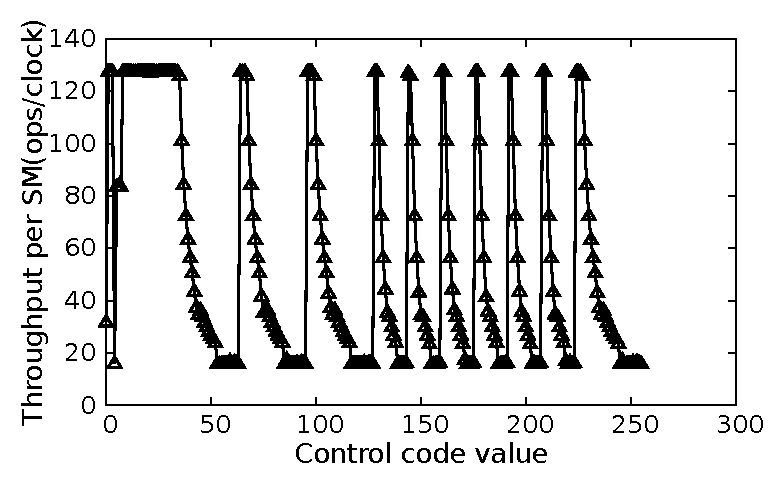
\includegraphics[width=2.1in]{ctrl}
       \subcaption{Regulate {\tt FFMA} throughput. \jled{8-bit control code value} \jled{ops/cycle? or IPC?}}
        \label{fig:control_throughput}
    \end{subfigure}
    \begin{subfigure}[htbp]{0.3\textwidth}
        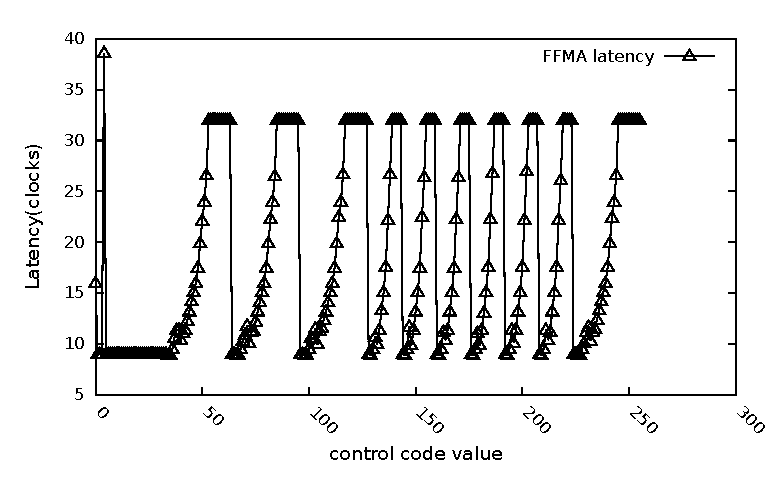
\includegraphics[width=2.1in]{ctrl_latency}
        \subcaption{Regulate {\tt FFMA} latency. \jled{8-bit control code value}}
        \label{fig:control_latency}
    \end{subfigure}
    \begin{subfigure}[htbp]{0.3\textwidth}
        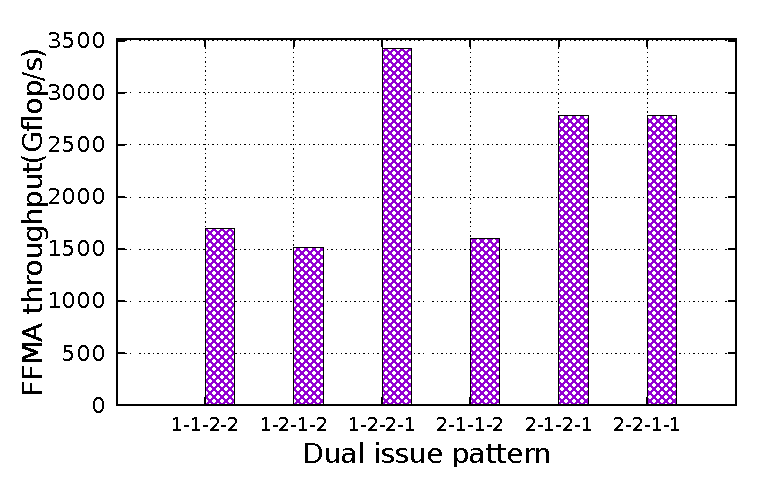
\includegraphics[width=2.1in]{pattern}
        \subcaption{Peak {\tt FFMA} throughput(S: single issue, D: dual issue). \jled{Y-axis is performance?}}
        \label{fig:control_pattern}
    \end{subfigure}
    \caption{Different control code impact on performance}
    \label{fig:control_code}
\end{figure*}


{\em {\bf Observation 1--[Control]}: 
Warp scheduling and issue mode are tunable by modifying control codes which regulate instruction execution.}

Starting with the Kepler architecture, NVIDIA has been moving some control logics off the chip and into kernel 
instructions which are determined by the assembler~\cite{lai,maxas}. This evolution provides programmers the opportunity to 
make globally optimal scheduling decisions and other control optimizations if an assembler is available. The disassembly code from sample programs and cuBLAS library indicates that every $64$-bit control binary code controls \jled{at most} $7$ instructions as Figure~\ref{fig:assemblycode}.
% a control code is placed before $7$ instructions, and it 
We identify that both the highest $6$ bits and lowest 
$2$ bits are {\em opcodes}, and the middle $56$ bits are used to control the execution of $7$ 
instructions, each of which is assigned to $8$ control bits.

For the $8$ control bits, we identify their meanings by statically examining the disassembly codes of cuBLAS and 
dynamically benchmarking instruction sequence of different control codes.
In this way, we discover bit-$4$ marks global memory dependency barrier, bit-$5$ represents shared memory dependency barrier, and bit-$7$ indicates a texture cache dependency barrier due to its weak consistent memory model. 
Some unexpected values are loaded if the any $4-7$ bits is not set. 
\jled{Wrong bit number, bit-4 not 4th bit! What about bit-$6$?? Please check the correctness.} 
% We verify the $7$\textsuperscript{th} bit of the control 
% code of {\tt TEXDEPBAR} instruction is set to $1$, to
% indicate a texture dependency barrier of texture cache due to its weak consistent memory model. 
We use {\tt FFMA} instruction's behaviors to crack $0-3$ bits of its control code.
Figure~\ref{fig:control_code}(\subref{fig:control_throughput}) and 
Figure~\ref{fig:control_code}(\subref{fig:control_latency}) show {\tt FFMA}'s throughput and latency  when its $8$ control bits varies from $0$ to $255$. 
% Thus, most throughputs achieve the maximum when the control code's value is smaller than {\tt 0x20} because of no set suspension.
% Obvious periodicity is shown with size $16$ after the control code's value reaches {\tt 0x20}.
After {\tt 0x20}, both the throughput and latency show obvious periodicity.
For each period, by increasing the value of $0-3$ bits, the {\tt FFMA} throughput drops and its latency raise by different rates. \jled{the period size is different! why?}
This phenomenon implies that the $4$ lower bits stores the number of stall cycles before issuing 
an instruction. 
Our microbenchmarking reveals some specific patterns of control codes:
% Furthermore, the microbenchmarking reveals some specific patterns of control codes:

\begin{itemize}
\item When the control bits are set to be {\tt 0x00}, the scheduler suspends a warp of the instructions for $16$ cycles.
\item {\tt 0x2n} means a warp is suspended for $n$ cycles before issuing the next instruction, where $n=0, \dots, 15$.
\item {\tt 0x00} means single issue mode, while {\tt 0x04} means dual-issue mode. 
While two consecutive instructions are controlled by {\tt 0x04} and {\tt 0x05} respectively, the throughput could reach the maximum. \jled{relation with Figure?}
\end{itemize}


{\em {\bf Observation 2--[Register]}: 
Irrespective of single- or dual-issue mode, only source operands may cause register bank conflicts that degrades instruction throughput.}

Shared memory bank conflict is well-known as an important performance factor for CUDA programming.
Recent research~\cite{lai} noticed that register bank conflict is also nontrivial to performance. 
In order to probe 
register bank conflict, our microbenchmark measures instruction throughput for different combination of {\tt FFMA} 
register operands. 
Table~\ref{tab:th} shows one example combination resulting in various efficiency numbers. 
The rightmost column represents the number of register bank conflicts recorded from our experiments. 
This experiment is conducted 
in single issue mode by setting control code to 0x20 \jled{0x00 is single-issue mode ?}. 
Theoretical, the peak efficiency is $128/192=66.67\%$ \jled{why 128?}. 
In fact, we observe that both single- and dual-issue mode produce the same throughput behavior for bank conflicts.
 % variance of instruction throughput. 
From our experiments on Kepler architecture, we observe:
\begin{itemize}
\item Destination operand will not contribute to bank conflict, no matter which bank is assigned to it.
\item When source operands have 2- or 3-way register bank conflict, the throughput will drop up to 2.33\% and 17.17\% respectively in single issue mode. 
% When source operands have 3-way conflicts, the throughput will drop by up to 17.17\%. 
    \jled{Is the two numbers fixed?}
\item Our microbenchmark finds out a proper distribution of registers to eliminate bank
     conflict. 
     The distribution is summarized in Table~\ref{tab:reg}, which confirms the rule in~\cite{lai}: \\
 bank0$\Leftarrow$($Ridx \% 8 < 4$ \&\& $Ridx \% 2 == 0$) \\
 bank2$\Leftarrow$($Ridx \% 8 < 4$ \&\& $Ridx \% 2 == 1$) \\
bank1$\Leftarrow$($Ridx \% 8 > 4$ \&\& $Ridx \%2 == 0$) \\
bank3$\Leftarrow$($Ridx \% 8 < 4$ \&\& $Ridx\% 2 == 1$)\\
where $Ridx$ is the register number. 
This rule will guide the performance tuning of SGEMM code.

\end{itemize}

\begin{table}[htbp]
    \caption{The efficiency of instruction throughput varies with difference register bank distribution. {\it Inst} : 
instruction pattern, {\it Th/SM}: the instruction throughput per SM, {\it Eff}: efficiency of throughput, {\tt Conf}: register bank conflicts.}
\centering
\scalebox{1.0} {
\begin{tabular}{|c|c|c|c|}
\hline
Inst &Th/SM&Eff&Conf\\
\hline
{\tt FFMA R5,R4,R1,R0}&127.50&66.40\%&0\\
\hline
{\tt FFMA R2,R4,R1,R0}&127.50&66.40\%&0\\
\hline
{\tt FFMA R5,R2,R1,R0}&119.18&62.07\%&2-way\\
\hline
{\tt FFMA R3,R2,R1,R0}&119.18&62.07\%&2-way\\
\hline
{\tt FFMA R5,R9,R3,R1}&94.52&49.23\%&3-way\\
\hline
{\tt FFMA R11,R9,R3,R1}&94.52&49.23\%&3-way\\
\hline
{\tt FMUL R4,R1,R0}&127.50&66.40\%&0\\
\hline
{\tt FMUL R4,R2,R0}&119.17&62.06\%&2-way\\
\hline
\end{tabular}
}
\label{tab:th}
\end{table}


\begin{table}[htbp]
\caption{Register bank distribution.}
\centering
\scalebox{1.0} {
\begin{tabular}{|c|c|c|c|c|c|c|c|c|}
\hline
    {\tt Bank0}&{\tt R0}&{\tt R2}&{\tt R8}&{\tt R10}&{\tt R16}&{\tt R18}&{\tt R24}&{\tt R26}\\
\hline
    {\tt Bank1}&{\tt R1}&{\tt R3}&{\tt R9}&{\tt R11}&{\tt R17}&{\tt R19}&{\tt R25}&{\tt R27} \\
\hline
    {\tt Bank2}&{\tt R4}&{\tt R6}&{\tt R12}&{\tt R14}&{\tt R20}&{\tt R22}&{\tt R28}&{\tt R30}\\
\hline
    {\tt Bank3}&{\tt R5}&{\tt R7}&{\tt R13}&{\tt R15}&{\tt R21}&{\tt R23}&{\tt R29}&{\tt R31}\\
\hline
\end{tabular}
}
\label{tab:reg}
\end{table}

{\em {\bf Observation 3--[Arithmetic]}: 
With a proper control code pattern and register allocation, {\tt FFMA} 
instruction throughput can approach the theoretical peak in dual issue mode.}

It's very intricate to tune instruction execution to improve instruction throughput. The previous work~\cite{lai} 
reports the maximal throughput of {\tt FFMA} per SM as $132$, which is much lower than the theoretical throughput ($192$) on Kepler. 
Our microbenchmark reveals several key points of optimization to approach theoretical peak on Kepler. 
First, the control code must be set properly to dual issue adjacent instructions. Second, the ratio and interval of 
dual issue {\tt FFMA} instructions must be tuned into a specific pattern. 
Since each warp of extra computing unit is 
shared among two warps, \jled{non clear} when all threads are trying to fully dual issue every two adjacent {\tt FFMA}s, half of the 
scheduler would stall due to computing resource conflict. 
Thus, the optimal ratio of dual issue to single issue is $2:2$ theoretically, and 
with a proper phase shift among two warp's executing pace, they could get access to the shared computing unit in turn. \jled{not clear}
Using the $2:2$ ratio, \( \begin{pmatrix} 4 \\ 2 \end{pmatrix} \) $=6$ combinations for mixed single  and dual issue pattern inside a $7$ instructions scheduling block (Figure~\ref{fig:control_code}(\subref{fig:control_pattern})). 
We choose the best {\tt SDDS} pattern in our SGEMM implementation. 
Third, the first instruction of the core loop needs to be aligned. This restriction is 
caused by the aligned position of control code in the instruction sequence. 
Last, {\tt FFMA} dual issue requires $6$ register banks from Table~\ref{tab:reg} \jled{Where is 6 from? Table~\ref{tab:reg}, right?}. 
Instruction order has to be adjusted to fully use Kepler's operand 
collector mechanism~\cite{collector,tarjan2012policy} to avoid register bank conflicts.
\jled{A new concept: operand collector mechanism. Maybe just don't mention it.}
As shown in 
Table~\ref{tab:ffma}, these optimizations together improve {\tt FFMA}'s throughput to $190$ ops/clock \jled{ops/cycle?}, which is very close to the theoretical peak $192$ ops/clock.

\begin{table}[htbp]
\caption{Floating-point instruction throughput on Kepler}
\centering
\scalebox{1.} {
\begin{tabular}{|c||c|c|c|}
\hline
Inst &operation&single issue&dual issue\\
\hline
{\tt FFMA} &c=a*b+c&127.52&190.35 \\
\hline
{\tt FMUL} &c=a*b&127.52&190.35 \\
\hline
{\tt FADD} &c=a+b&127.52&191.50\\
\hline
\end{tabular}
}
\label{tab:ffma}
\end{table}


{\em {\bf Observation 4--[Memory]}: For higher memory bandwidth, shared memory prefers 64-bit load 
instruction {\tt LDS.64} while global memory prefers the load instruction with texture cache {\tt LDG}.}

For GPU memory hierarchy we focus on the programmer controllable memory resources, shared memory and global memory. 
On NVIDIA GPU architecture, there are different memory access widths (32-bit, 64-bit, 128-bit) and paths (through normal or texture cache). 
In fact, both NVIDIA documents and previous studies~\cite{tan} pointed out that wider 
instructions have longer pipeline latency.
Our benchmarking confirms this phenomenon and also identifies several bandwidth issues for memory optimization.


\jled{operations refer to instructions here?}
Intuitively, a wider load operation should achieve higher bandwidth. 
We test the bandwidth of shared memory operations with different widths, {\tt LDS.32}, {\tt LDS.64},
and {\tt LDS.128}. 
The operations are specially arranged to avoid shared memory bank conflict. 
% In this experiment, the amount of data are projected to the number of load instructions. 
Assume the data can be loaded by $N$ {\tt LDS.128} instructions, 
then $2N$ {\tt LDS.64} or $4N$ {\tt LDS.32} instructions are needed.
Figure~\ref{fig:lds_bw} compares the sequential memory access bandwidth of the three instructions by increasing the data volume. 
{\tt LDS.64} achieves the highest bandwidth $137GB/s$, which is about $76\%$ of the peak bandwidth\footnote{The 
theoretical shared memory bandwidth for each SM can be calculated as $Bandwidth = f_{core} \times Width \times Warpsize$ in
bytes, where $f_{core}$ is the frequency of a CUDA core, $Width$ is bank width, $Warpsize$ is warp size.}.

\begin{figure}[htbp]
\begin{center}
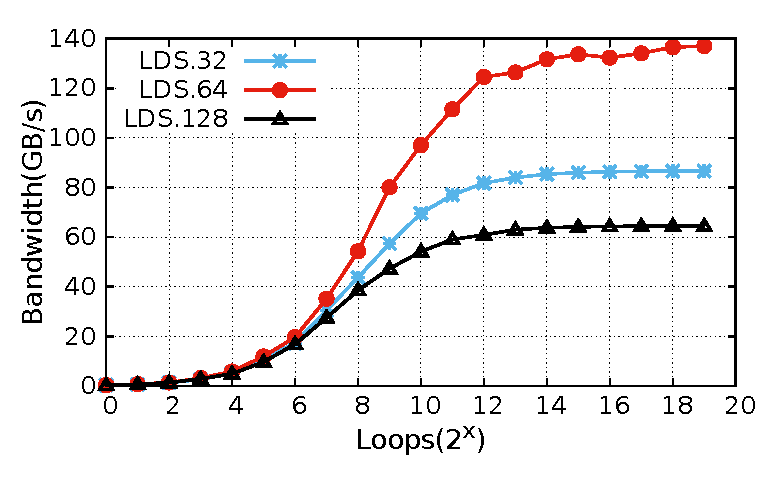
\includegraphics[scale=0.6]{lds_bandwidth}
    \caption{ Bandwidth of {\tt LDS.32}, {\tt LDS.64} and {\tt LDS.128}}
\label{fig:lds_bw}
\end{center}
\end{figure}

% global memory
Two paths are used to load data from global memory, through L2 cache by {\tt
LD} instruction or through texture cache by {\tt LDG} instruction. 
We launch $26$ thread blocks each with $512$ threads, and specifies that each thread accesses $4$ words in a stride of $4 \times blockDim.x \times gridDim.x$. 
Our benchmark confirms that {\tt LDG} achieves higher bandwidth than {\tt LD}.
% , which has been identified by previous work~\cite{tan}.


\section{Applying Optimizations to SGEMM}
\label{sec:optimization}
The demystified GPU microarchitecture features provides additional space to tune performance-critical kernels. We apply a series of incremental optimizations to improve SGEMM efficiency on Kepler architecture. The optimization strategies go through architectural hierarchy from core and register to memory. All the optimization strategies are inspired by our microbenchmark's observations.
\begin{itemize}
\item At core level, we orchestrate {\tt FFMA} instruction executions by a more efficient instruction scheduling pattern with respect to the proper control code.
\item At register level, we meticulously map operands to registers so that  bank conflicts are avoided in the inner loop iteration.
\item At memory level, we select appropriate shared memory load/store width and global memory data path to mitigate latencies.
\end{itemize}

\subsection{Instruction Scheduling}
\subsubsection{Schedule {\tt FFMA} Instructions}
It's ideal to keep warp scheduler dual issue instructions (i.e., {\tt FFMA}) all the time. However, for each SM on Kepler architecture, 64 cores share $4$ schedulers, each of which issues instructions to 32 cores as a warp. As noted in {\em observation 3}, the best pattern of {\tt FFMA} instructions block is a sequence of 2 dual issues (4 {\tt FFMA}s) and 2 single issues ((2 {\tt FFMA}s)). As shown in Figure~\ref{fig:assemblycode}, the instructions in lines 2-3 and lines 5-6 are respectively grouped as two dual-issues. The other two instructions in line 8 and line 11 are two single issues in terms of floating-point instruction execution. As a comparison, most of the {\tt FFMA}s are single-issues in the CUDA compiler generated codes.

\begin{figure*}[htbp]
\begin{center}
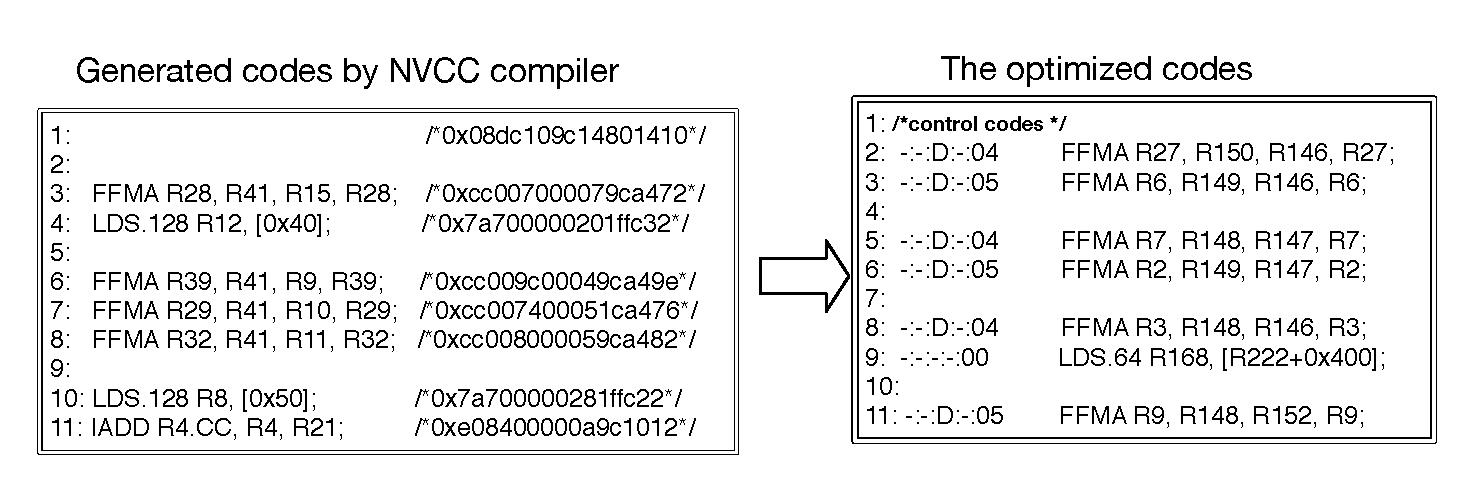
\includegraphics[scale=0.6]{assemlycode}
    \caption{The comparison of compiler generated codes and our tuned assembly codes.}
\label{fig:assemblycode}
\end{center}
\end{figure*}

\begin{figure}[htbp]
\begin{center}
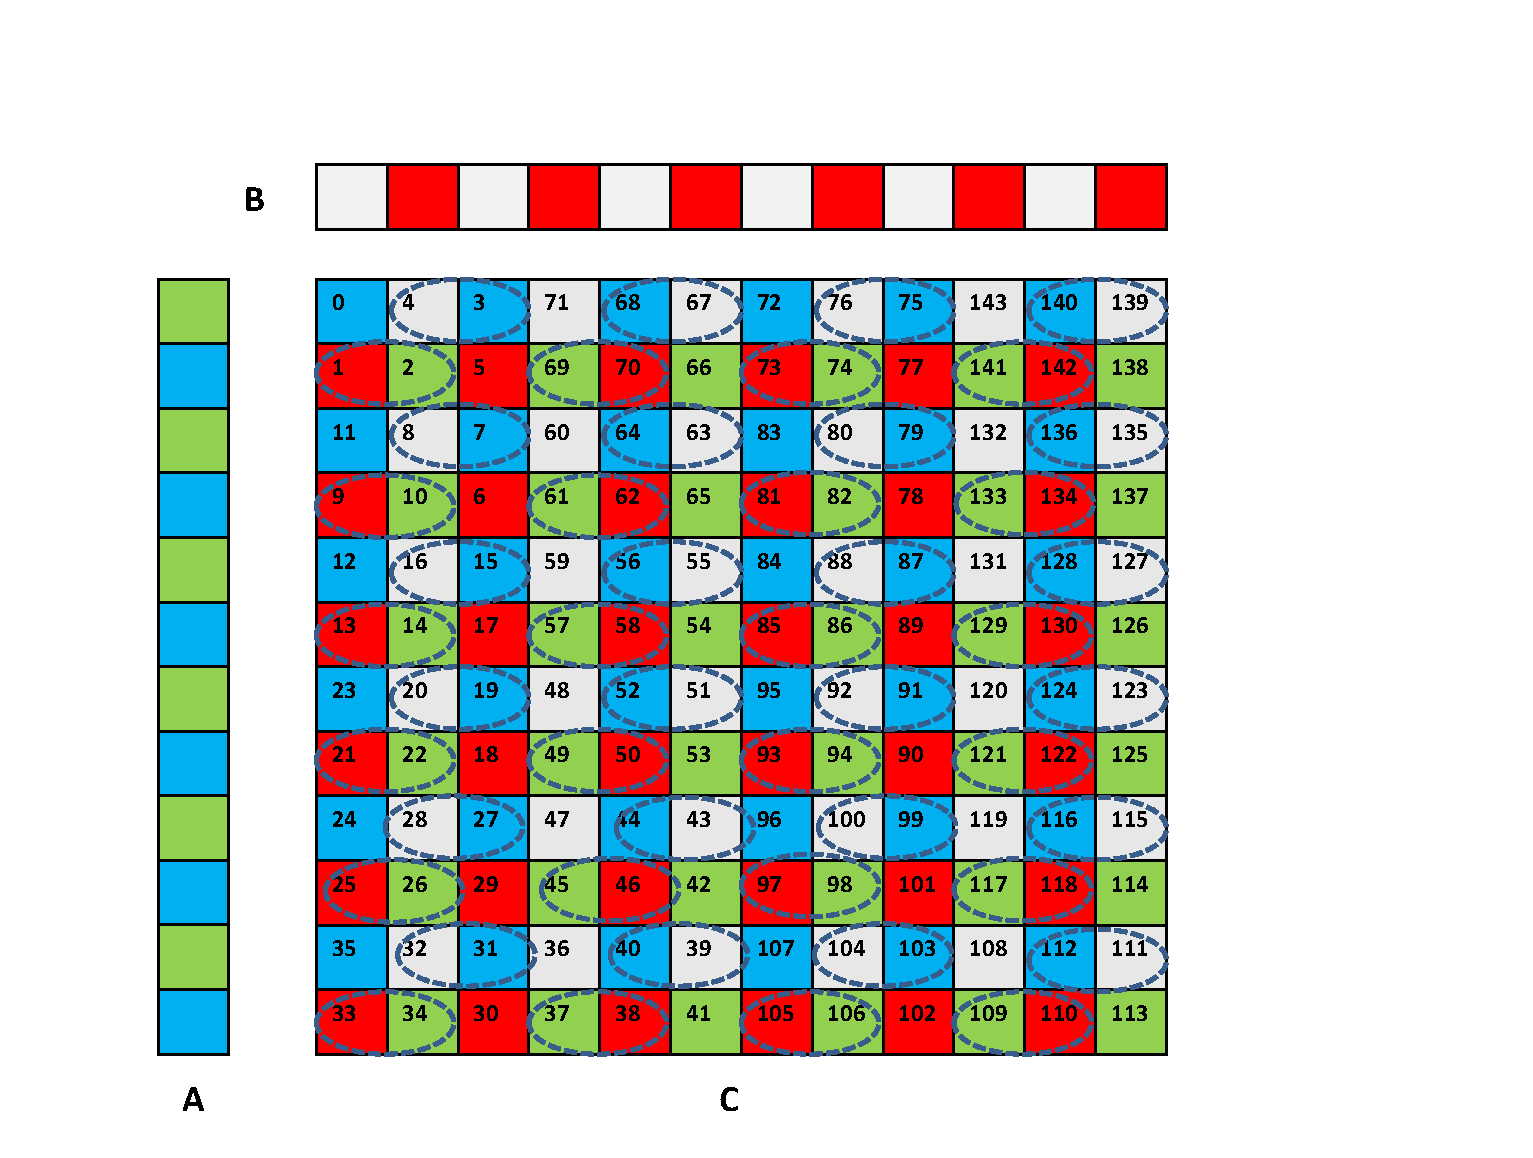
\includegraphics[scale=0.5]{order}
\caption{{\tt FFMA}s instructions scheduling for calculating a $12\times 12$ subblock of matrix C.  The numbers in cells denote {\tt FFMA} execution order. Dashed ellipses across two cells mean that two {\tt FFMA} instructions are executed at same clock cycle.}
\label{fig:order}
\end{center}
\end{figure}

Based on the basic {\tt FFMA} instruction block, the scheduling pattern is depicted in Figure~\ref{fig:order}, which
illustrates the order of $144$ {\tt FFMA}s instruction execution for calculating a $12\times 12$ subblock of matrix C.
For example, the {\tt FFMA} to calculate $c_{00}$ is the first instruction to be issued. Then, both {\tt FFMA}s to
calculate $c_{10}$ and  $c_{11}$ are simultaneously issued. We arrange all the {\tt FFMA} operations according to issue
order illustrated in Figure~\ref{fig:order}.

Another advantage of this execution order is less register pressure due to register data reuse, which can facilitate
operand collector mechanism~\cite{collector}. Operand collector is storage element coupled from register file and
provides inputs to the data path of the processor core for executing an instruction. Operands may be cached and reused
in the subsequent instructions. The assembly code in Algorithm~\ref{fig:order} lists the instructions to calculate
$C_{22}, C_{21}, C_{30}, C_{31}, C_{20}, C_{40}$, where are corresponding to the orders of $7,8,9,10,11,12$ in
Figure~\ref{fig:reg}. The reuse happens as follows. The {\tt FFMA} in line 2 uses the cached operand {\tt R150} from the previous instruction block. Line 3 uses the cached operand {\tt R146} from the previous instruction. Similarly, The {\tt FFMA} in line 6 reuses the cached operands of   {\tt R149} and {\tt R147} from the previous two instructions, respectively.

\begin{table}[!t]
\caption{The position table of {\tt Non-FFMA} instructions. The inner-loop is unrolled by 4 times. The first column records slot numbers.}
\label{tab:position}
\captionsetup{font=scriptsize}
\centering
\scalebox{0.78} {
\begin{tabular}{|c|c|c|c|c|}
\hline
\diagbox[width=4em, height=3em]{slot}{unroll} & 0 &1 &2 &3 \\
    \hline
    5 & ISET P0 & IADD A0 & & XOR smB \\
    \hline
    11 & LDS.64 smA & LDS.64 smA & LDS.64 smA & LDS.64 smA \\
    \hline
    17 & LDS.64 smA & LDS.64 smA & LDS.64 smA & LDS.64 smA \\
    \hline
    23 & LDS.64 smA & LDS.64 smA & LDS.64 smA & LDS.64 smA \\
    \hline
    29 & LDS.64 smA & LDS.64 smA & LDS.64 smA & LDS.64 smA \\
    \hline
    35& IADD K, -4 & IADD A1 & TEXDEPBAR & \\
    \hline
    41 & LDS.64 smB & LDS.64 smB & LDS.64 smB & LDS.64 smB \\
    \hline
    47 & LDS.64 smB & LDS.64 smB & LDS.64 smB & LDS.64 smB \\
    \hline
    53 & LDS.64 smB & LDS.64 smB & LDS.64 smB & LDS.64 smB \\
    \hline
    59 & LDS.64 smB & LDS.64 smB & LDS.64 smB & LDS.64 smB \\
    \hline
    65 & & &STS.64 writeS & ISETP P2 \\
    \hline
    71 & & & & \\
    \hline
    77 & & IADD B0 & & LDG A \\
    \hline
    83 & LDS.64 smA & LDS.64 smA & LDS.64 smA & LDS.64 smA \\
    \hline
    89 &ISETP P3 & & &\\
    \hline
    95 & LDS.64 smA & LDS.64 smA & LDS.64 smA & LDS.64 smA \\
    \hline
    101 & & & STS.64 loadB0 & LDG B \\
    \hline
    107 & & & STS.64 loadB2 & XOR writeS \\
    \hline
    113 & & & & \\
    \hline
    119 & LDS.64 smB & LDS.64 smB & LDS.64 smB & LDS.64 smB \\
    \hline
    125 & & & XOR smA & \\
    \hline
    131 & LDS.64 smB & LDS.64 smB & LDS.64 smB & LDS.64 smB \\
    \hline
    137 & & & & \\
    \hline
    143 & & IADD B1 & BAR.SYNC & BAR Loop \\
    \hline
\end{tabular}
}

\end{table}

\subsubsection{Schedule {\tt non-FFMA} Instructions}

After setting the order of {\tt FFMA}, other {\tt non-FFMA} instructions should be inserted in proper positions to assure
corretness of the program without losing performance. In order to tolerate instruction latency, we need to keep distance of dependent instructions to be larger than the latency. The distance can be approximately computed as
\begin{displaymath}
distance = \frac{4\times\#instructions}{7}
\end{displaymath}
In a schedule block, there are $7$ instructions which cost $4$ clocks to be issued in dual issue mode. In other word, if we want to have interleave
two instructions of $L$ distance, then $\frac{L*7}{4}$ instructions are needed. Besides, the remained number of slots to insert these instructions is estimated as follows:

\begin{displaymath}
\#slots = \frac{bm\times bn\times unroll}{ffmas\_in\_schedule\_block}=\frac{12\times 12\times 4}{6}=24\times 4
\end{displaymath}

According to these principles, we first arrange {\tt LDS}, {\tt STS}, {\tt LDG} due to their long latencies. The
schedule slots are illustrated in two dimension as shown in Table~\ref{tab:position}.
Note that we use double buffers to hide latency of {\tt LDG} from global memory, which costs $200$ clock cycles.
Every $4$ loop requires $2$ {\tt LDG}s to load data from global memory to registers, $4$ {\tt STS}s to store data from registers to shared memory. There is a read after write (RAW) dependency between {\tt
LDG} and {\tt STS}. The simple model estimates that $\frac{200\times 7}{4} = 350$ are needed instructions between them.
As shown in Table~\ref{tab:position}, we put {\tt LDG} and  {\tt STS} in position $P[77][3]$ and position $P[65][2]$, respectively. Thus, the number of instructions between them are $143-77 + 144\times 2 +
65=419$, resulting in a distance of $\frac{4\times 419}{7}=239$ clocks, which is enough to hide latency of {\tt LDG}s.

The arrangement of {\tt LDS}s, which load data from shared memory for double buffers of both $A$ and $B$, follows the same way with {\tt LDG}s.
A {\tt LDS} has a latency of $40$ clock cycles, $\frac{40\times 7}{4}=70$ instructions are needed to interleave {\tt LDS} and {\tt
FFMA}. As shown in Table~\ref{tab:position}, {\tt LDS} in $P[11][3]$ read data from {\tt STS} in position $P[65][2]$, the distance is more than $40$ clock
cycles. In the end, a {\tt BAR.SYNC} should be inserted after {\tt STS} before {\tt LDS} to make sure that data in shared memory is ready. Other instructions like {\tt XOR},
{\tt IADD}, {\tt ISETP} are inserted according to data dependency, there is almost no performance loss due to little latency.


\subsection{Register Allocation}

To allocate register for $A$ column, $B$ row and $C$ submatrix, we have three considerations: correctness, no bank
conflict and allocate register index tightly.
{\tt LDG.128} restricts $4$ words alignment restriction for register.
Nvidia GPU does not have $128$ bit register, in order to use $128$ bit load, one destination register $RN$ is given, result is writen to
$RN+1$, $RN+2$, $RN+3$. There is undocumented restriction: $N\%4==0$, otherwise illegal instruction error will be reported.
It's not hard to understand this restriction, $4$ words align for {\tt LDG.128} make hardware logic simpler saving die area.
Since we will use {\tt LDG.128} to load $A$ and $B$, there are $2$ bank allocation choices due to $N\%4==0$ restriction and
bank distribution of Kepler. We assume allocate $A$ matrix bank $\begin{bmatrix} 0 \\ 1  \end{bmatrix}$,
$B$ bank $\begin{bmatrix} 2 & 3 \end{bmatrix}$ as shown in Figure, we have 2 choices left for $C$.
$\begin{bmatrix} 1 & 2 \\ 3 & 0  \end{bmatrix}$
$\begin{bmatrix} 3 & 1 \\ 0 & 2  \end{bmatrix}$
We have $2i\times2$ bank patterns for SGEMM, we choose $\begin{bmatrix} 0 \\ 1  \end{bmatrix}$ $\begin{bmatrix} 2 & 3 \end{bmatrix}$
$\begin{bmatrix} 1 & 2 \\ 3 & 0  \end{bmatrix}$ for $A$, $B$ and $C$ respectively as shown in Figure.
To allocate actual register index, we choose continuous register index so that register index do not get too big to
exceed 255 restriction. From figure, we can verify that $C_{ij}$, $A_i$ and $B_j$ have different banks, for example
$C_{01}$'s color is white, $A_0$'s color is green and $B_1$'s color is red, hence no bank conflicts.

\begin{figure}[htbp]
\begin{center}
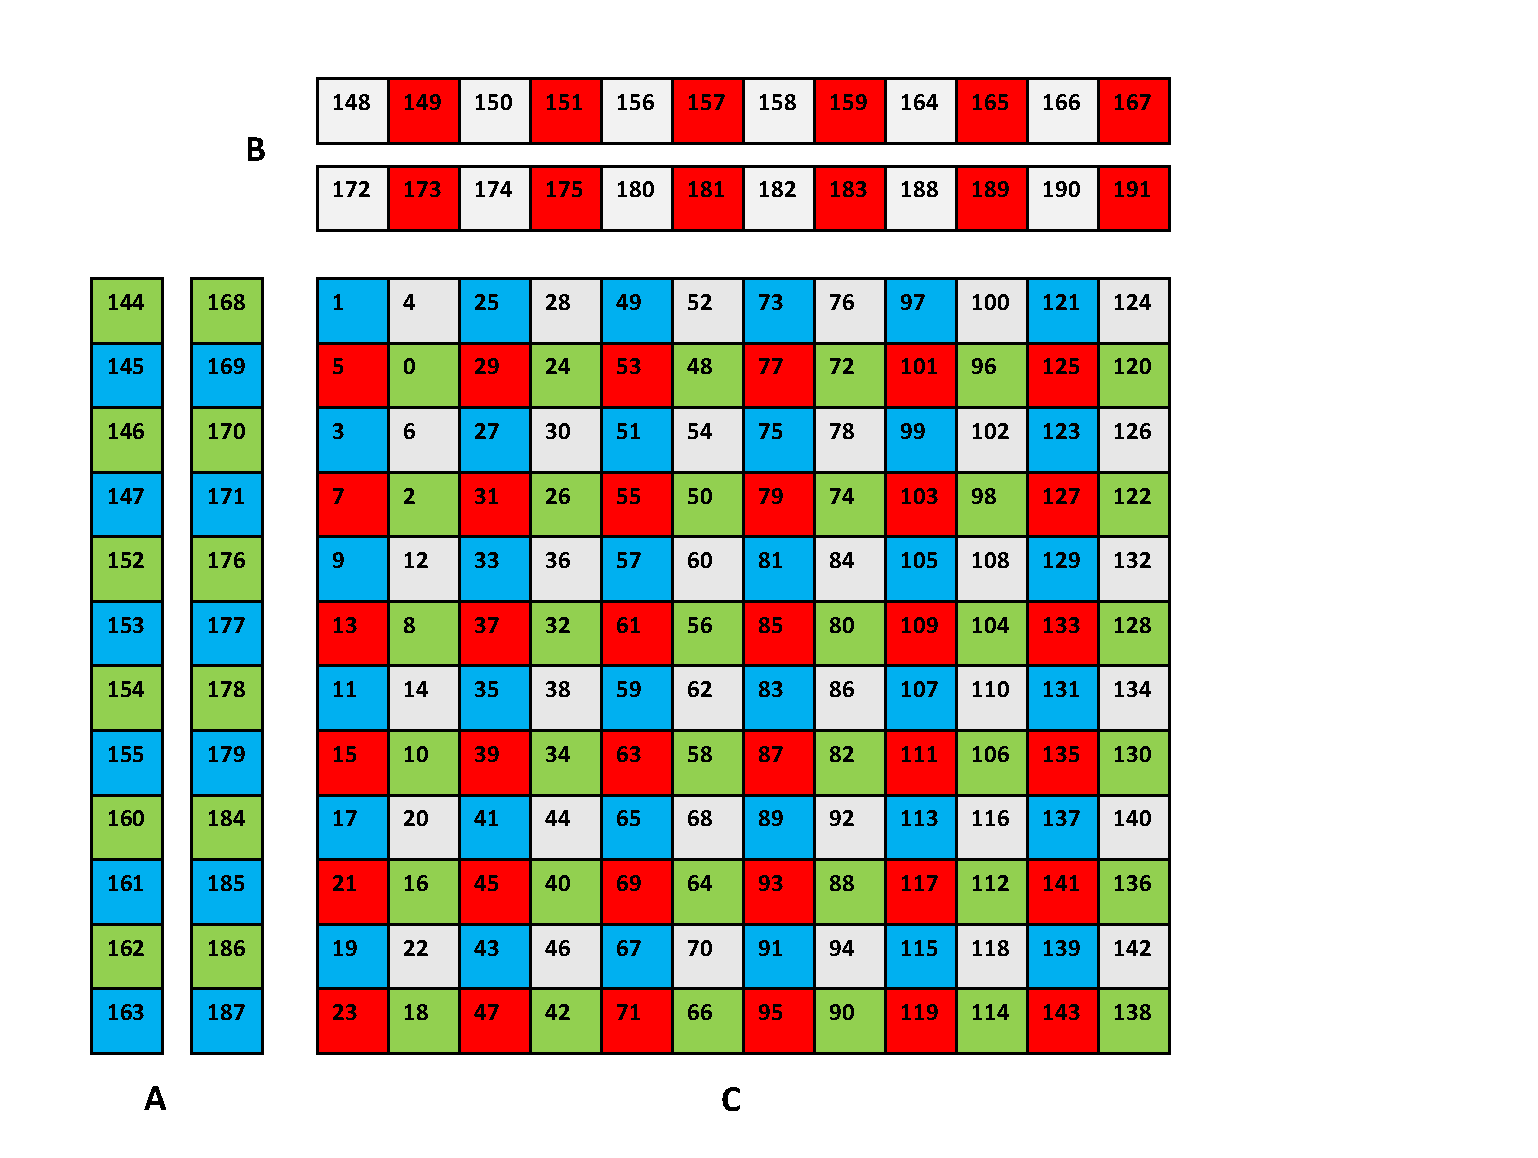
\includegraphics[scale=0.55]{reg}
\caption{An illustration of register bank allocation. The number in the cell is register number. Double buffering column
    $A$ and row $B$. The leftmost two columns of registers are allocated to one column of $A$ sub-matrix, the
top two rows of registers are allocated to one row of sub-matrix $B$, others are registers for
sub-matrix $C$. The different colors denotes mapping of register banks: Green$\rightarrow$bank0, blue$\rightarrow$bank1, gray$\rightarrow$bank2, red$\rightarrow$bank3.}
\label{fig:reg}
\end{center}
\end{figure}


\subsection{Memory Movment}
According to the optimization observation on memory access suggested by microbenchmark, we use {\tt LDS.64} to load data from shared memory and {\tt LDG.E.128} to load data from global memory. Specifically we have additional reasons to adopt them in SGEMM kernel. First, the use of {\tt LDG.E.128} can reduce the number of {\tt non-FFMA} instructions. For example,  in the inner loop, the number of 32-bits load operations to read $A$ and $B$ is 12. The wider {\tt LDG.E.128} operation reduces the numbers to be 3.

Second, it is another story for shared memory. The shared memory transaction size of 256 bytes forces that any shared memory request will be split into multiple transactions of 256 bytes. By inspecting the inner loop, we cannot control when the second transactions happen so that it is difficult to eliminate potential bank conflicts between {\tt LDS.128}s and {\tt FFMA}s. As for {\tt LDS.64}, it's determinable to avoid register bank since a transaction just happens at the position of {\tt LDS.64}.


\section{Evaluation}

In this section, we compare the optimized SGEMM performance in Gflop/s with NVIDIA CUBLAS. The $12\sim 25\%$ improvement shows that the microarchitectural optimization makes sense of tuning SGEMM on GPUs.   We further present a quantitative analysis of the effect of each individual optimization strategy and an estimation of the upper bound performance.

The experiments are conducted on NVIDIA K20m GPU, which hardware configuration is summarized in Table~\ref{table:k20}. The compared CUBLAS is from CUDA $7.0$ version. In our experiments the sizes of matrix vary in $768\times768$, $1536\times1536$,$3072\times3072$,$6144\times6144$,$12288\times12288$.

\begin{table}[!t]
\caption{The configuration of NVIDIA Tesla K20m GPU.}
\centering
\scalebox{1.0} {
\begin{tabular}{|c||c|}
\hline
Metric& Value\\
\hline
SPs/SM &192\\
\hline
    SMs&13\\
\hline
Cores &2496\\
\hline
Frequency(MHz)&705\\
\hline
Memory Bus Width&320\\
\hline
Memory frequency&2600 Mhz\\
\hline
Bandwidth(GB/s)&208.0\\
\hline
Single FLOPS&3520\\
\hline
warp schedular per SM&4\\
\hline
dispatch unit/SM&8\\
\hline
Max registers/thread&256 \\
\hline
32-bit registers/SM&64K\\
\hline
LD/ST unit&32 \\
\hline
shared memory&48KB\\
\hline
L1 cache&16KB or 48KB\\
\hline
    L2 cache&1536KB\\
\hline
\end{tabular}
}
\label{table:k20}
\end{table}


\subsection{Overall Performance}
Figure~\ref{fig:sgemm_tn} reports the performance comparison of CUBLAS SGEMM and our optimized SGEMM.
Our SGEMM achieves $3104$ Gflop/s which efficiency is $3104/3520=88\%$. With the same matrix size, CUBLAS has $2216$ Gflop/s which efficiency is $63\%$. The comparison shows that our implementation achives 25\% performance improvement over CUBLAS.

As the figure shows, the overall trend is that performance increases with bigger matrices. On one hand, the larger matrix size leads to a higher ratio of floating-point operations to memory operations, which is more close to the hardware arithmetic intensity. On the other hand, the larger matrix size increases occupation of the threading CUDA cores. The numbers of block ranges from $[768/192,768/192]=[4,4]$ to $[12288/192, 12288/192]$ $=[64,64]$. Since Kepler has $13$ SMs in total, matrix of size $768\times 768$ suffers from low utilization of massive cores. Therefore, we observe that there is significant growth in Gflop/s from 768 to 1536 for both ours and CUBLAS. With respect to the ratio of performance improvement, the optimization has less effect on the smaller matrix size than the larger one. The reason is that the performance is increasingly bounded by the microarchitecture rather than memory due to the higher arithmetic intensity. Thus, our microarchitecture-level optimization plays more important role on tuning performance.

\begin{figure}[htbp]
\begin{center}
\includegraphics[scale=0.6]{sgemm_tn}
\caption{Performance comparison of CUBLAS and the optimized SGEMM }
\label{fig:sgemm_tn}
\end{center}
\end{figure}

\subsection{Performance Analysis}

\subsubsection{Profiling Microarchitectural Optimization}
In order to examine performance gain of different optimization strategies, we construct several intermediate implementations by incrementally applying the microarchitectural optimizations.

{\it Baseline:}~~The baseline involves conventional optimizations including register blocking, global
memory double buffer, shared memory double buffer and unrolling, rather than assembly level optimization.
For example, baseline use default $32-bit$ {\tt LD} rather than $128-bit$ {\tt LDG} to load data from global memory.
Register allocation for $C$ is allocated orderly from $0$ to $143$, then $A$ and $B$ matrices. In this case, {\tt
FFMA}s will have $368/(144*4)=63.89\%$ and $64/(144*4)=11.11\%$ 3-way bank conflicts. Baseline does not apply dual
issue optimization either.

{\it +Reg:}~~The register allocation pattern described in section~\ref{sec:assembler} is applied to eliminate register bank conflict. No
instruction scheduling change between this version and baseline version.

{\it +LD128:}~~Use wider global load instruction.
Kepler has an L1 data cache, but it is designed for local rather than global memory access. So {\tt LD} will not be L1-cached, it may be L2-cached.

{\it +LDG128:}~~{\tt LD} is load instruction used in implementation. When {\tt LDG} is used, a {\tt TEXDEPBAR}~\cite{lukyanov2014efficient} is needed before using the data.

{\it +Dual:}~~Single issue is controlled by setting control code to $0x00$. Dual issue is fully enabled by utilizing the
pattern described in section~\ref{sec:assembler}. For dual issue version, $NOP$ may be inserted for instruction alignment.

\begin{figure}[htbp]
\begin{center}
\includegraphics[scale=0.65]{tn_prof}
    \caption{Evaluation of the incremental optimizations.}
\label{fig:th_prof}
\end{center}
\end{figure}

Figure~\ref{fig:th_prof} illustrates performance gain of each optimization method.
As long as number of instructions is changed, instruction order needs reschedual to achive high peformance.
Compared with the baseline implementation, $2.6X$ speedups are gained by applying all the optimization.

\section{Generality}
\label{sec:generality}

Although this paper examines the methodology as depicted in Figure~\ref{fig:workflow} on Kepler architecture and shows its performance optimizations for SGEMM, we argue that the developed toolchain can be easily extended to other NVIDIA GPUs and the explored optimization strategies is applicable to other floating-point computation-intensive applications.

{\em {\bf Generality of toolchain}}: For a given new GPU architecture, users only need to regenerated disassembly codes with CUDA binary utilities, and then feed them to the solvers, which are portable among different GPU architecture. We have validated the functionalities of the solvers on Fermi, Kepler, Maxwell and Pascal GPUs. The new assembler can be obtained by modifying the instruction grammar definition decoded by the solvers. In fact, this modification can be automatically generated with an assembler template~\cite{}. 

{\em {\bf Generality of optimizations}}: The optimization strategies include register allocation, memory load/store width and FFMA dual-issue. First, the former two strategies are applicable to other GPU architectures by leveraging the benchmark to detect effective patterns. Only is the third one specific to Kepler architecture. 

Second, note that the optimizations are microarchitectural specific rather than application specific. In fact, the previous investigations of GEMM optimization on CPU have inspired general performance tuning and compiler optimizations~\cite{lam1991cache}.  
Usually, the float computation-intensive applications can implemented using two hierarchy blocking:shared memory blocking and register blocking to hide latency of memory access and improve computation memory access ratio on GPU. As long long we use register blocking, there will be multiple float computation instructions inside the loop, then register allocation  and dual issue can refer our SGEMM's implementation in order to improve float computation throughput. For instance, the convolution algorithm in deep learning using $128\times128$ shared memory blocking and $8\times8$ register blocking, the register allocation can be derived by our bank patterns, and FFMA dual issue can use our 1-2-2-1 pattern. The {\tt LDG.128} can reduce number of memory instructions, continous memory access pattern applications can use this as well.
{\tt LDS.64} is best on Kepler due to the shared memory bank. We also vertified these two memory instruction achieve best for convolution algorithm.
The scheduling strategy is totally derived from instructions dependency,
which is not specific to SGEMM. Although we use a exhaust search method to search the optimal scheduling, we
argue that the idea may be applicable to general optimizations
because small piece of code often occupy most of the
execution time in a lot of scientific and engineering applications.
As an alternative way, auto-tuning techniques~\cite{} 
can be taken to find a better scheduling order. The instruction
scheduling optimization requires support of assemble language.
%For another floating-point intensive algorithm like convolution in deep learning applications, the FFMA throughput can be improved by eliminating register bank conflicts and activating dual issue. Then non-FFMA instructions are carefully scheduled without affecting the FFMA throughput. 
\begin{figure}[htbp]
\begin{center}
\includegraphics[scale=0.5]{cudnn}
\caption{cudnn vs convolution}
\label{fig:sgemm_tn}
\end{center}
\end{figure}

\section{Related Work}
To our knowledge, this paper provides the first comprehensive study of demystifying NVIDIA GPU microarchitecture which is correlated with performance tuning in SGEMM. This section briefly discusses related work in assembler, microbenchmarking and SGEMM optimization.

The lack of assembler for public use motivates a series of work on developing toolchains to facilitate tuning codes in assembly level. For the early architecture G80, Decuda~\cite{decuda} demonstrated the feasibility to operate the limited number of assembly instructions. Then, for almost each new generation of CUDA architecture, there are several efforts on developing assembly toolchains. Both Hou's Asfermi~\cite{asfermi} and Bernstein's cudaasm-qhasm~\cite{bernstein2012usable} are assemblers for Fermi architecture. Gray built MaxAs~\cite{maxas} assembler for Maxwell architecture by reverse engineering the encoding of Maxwell GPU. Our work provide a complete assembler for Kepler architecture. A remarkable advantage of our assembly toolchain is the compatibility with CUDA's {\tt cuobjdump}. As a comparison, although Envytools~\cite{envytools} supports PTX instruction translated to binary 64 bit instructions, it cannot generate a compatible {\tt cubin} format which directly used by the CUDA driver APIs. Besides, no prior work presents the detailed instruction solver algorithms as ours.

We share the same idea of performance microbenchmarking with other works. Wong et.al.~\cite{wong} performed a comprehensive benchmarking work on GT200 and provided pipeline latency data and
memory feature. Mei~\cite{mei} benchmarked memory hierachy
of Fermi, Kepler and Maxwell GPU, which including cache, shared memory etc. However neither of them benchmarked vectorized load instruction like {\tt LD} and {\tt LDS}. Due to lack of considering vectorized load instructions and too less instruction inside loop, the results is not so accurate. Neither of them considered dual issue modes of arithmetic instructions. We leverage the our complete assembler to crack control codes which reveal more microarchitecture details.

With respect to GEMM optimization in microarchitectural level, there are several work which inspires the implementation on specific GPUs. For example, we adopt the proved effective optimization techniques like shared memory/register blocking and double-buffering\cite{volkov}~\cite{tan}. Further, Tan et.al.~\cite{tan} implemented fast DGEMM by using assembly level optimization, such as software pipelining, vector memory operations, instruction scheduling. Lai~\cite{lai} presented performance analysis and optimization work of SGEMM on both Fermi and GTX680 GPUs. However, they don't consider dual issue mode by setting control code, which can boost performance significantly. Scott Gray~\cite{nervana_sgemm_wiki} presented optimization of SGEMM in assembly on Maxwell GPU. Since Maxwell does not support {\tt FFMA} dual issue, the optimization is much easier than
Kepler. In fact, we present a more complete case of applying microarchitectural features by combining instruction scheduling, register allocation and memory access paths.

\section{Conclusion}
\label{sec:conclusion}
We presented a methodology to demystify GPU's microarchitecture level features and demonstrated its 
application on tuning SGEMM. The methodology relies on a reverse engineering approach to crack the instruction encoding 
of GPU architecture, and a profound microbenchmarking at assembly level to correlate architecture features with 
performance factors, such as dual issue impact on float arithmetic throughput, memory load width on bandwidth, register 
bank distribution on performance etc. These parameters are worthwhile for both hardware and software researchers to 
understand GPU architecture and program optimization on GPUs. To our best knowledge, this is the 
first time to describe a detailed decoding solver to crack the instruction encoding. 
This solver is not limited to Kepler GPU, it can be easily applied to other GPU architectures. % \jled{``automatically'' change to easily}.

Based on the disclosed correlation between GPU architecture features and program performance, we implemented the optimized SGEMM in $3104$ Gflop/s with $88\%$ efficiency on Kepler GPU, which is $17\%$ higher than cuBLAS. 
We build two roofline models for shared and global memory separately, which reveal that even for compute-intensive SGEMM kernel, without appropriately optimizations or good resource usage, its performance could also be memory-bound.
Our work opens a door to optimize NVIDIA GPU code at native machine level, which may enlighten some optimizations on compilers or other computational kernels.
In future, we will apply our methodology to the latest Pascal GPU to revail GPU architecture features.
We also try to apply our insights of GPU microarchitecture to optimize code generation of open source GPU compiler
GPUCC~\cite{wu2016gpucc}.
%We also considering 
%Our future work is to extend this methodology to FFT and integrate optimized SGEMM into deep learning algorithms, such as convolutional neural networks (CNN).
%\jled{I added the future work. Please check or remove it.}
% cuBLAS's SGEMM achieves $2509$ Gflop/s ($71\%$ efficiency). 
% Our optimized one is $17\%$ higher than Cublas. 
% The performance boost is achieved on the basis of tuning {\tt FFMA} throughput as high as 
% hardware peak, then add other non-FFMA instruction with little penalty. 
% These optimizations include register bank 
% conflict eliminating, {\tt FFMA} dual issue scheduling, choosing proper width of global load and shared memory load instructions and so on.
%\jled{I removed one and a half unnecessary paragraphs.}
% Although Kepler is not the latest GPU, the arithmetic dual-issue feature will not be outdated.
% During our exploring of the way to fully exploit the arithmetic dual-issue feature of Kepler, we discovered that NVCC
% can not generate dual issue code efficiently which prohibits future GPU to adopt dual issue design. 
% However when scalability of thread level parallelism
% and frequency of GPU are too hard to improve, dual-issue feature would return in future GPU design.
% The development of GPU compiler could learn experiences from these microarchitectural-level optimizations.

%
% The following two commands are all you need in the
% initial runs of your .tex file to
% produce the bibliography for the citations in your paper.
%\bibliographystyle{abbrvnat}
\bibliographystyle{plain}

% The bibliography should be embedded for final submission.

\bibliography{bib/ref}
\newpage
\newpage
\pagebreak

\appendix
\section{Artifact description}

%Submission and reviewing guidelines and methodology: \\
%{\em http://cTuning.org/ae/submission-20160509.html}

%%%%%%%%%%%%%%%%%%%%%%%%%%%%%%%%%%%%%%%%%%%%%%%%%%%%%%%%%%%%%%%%%%%%%
\subsection{Abstract}

The artifact contains three parts of our work: KeplerAs assembler, optimized SGEMM code, and reverse-engineering GPU ISA encoding code. It can support the Algorithm $2$, $3$ and Figure $9$, $10$ in our PPoPP 2017 paper: Demystifying GPU Microarchitecture to Tune SGEMM Performance. To validate the results, run the test scripts and check the results in the according text output files.

%%%%%%%%%%%%%%%%%%%%%%%%%%%%%%%%%%%%%%%%%%%%%%%%%%%%%%%%%%%%%%%%%%%%%
\subsection{Description}

\subsubsection{Check-list (artifact meta information)}
%{\em Fill in whatever is applicable with some informal keywords and remove the rest}

{\small
\begin{itemize}
  \item {\bf Algorithm: SGEMM algorithm, KeplerAs assembler, GPU ISA encoding solver}
  \item {\bf Program: CUDA, C/C++ code, python and GPU assembly code}
  \item {\bf Compilation: nvcc, g++, python,perl and KeplerAs.pl (after install our GPU assembler KeplerAs)}
  %\item {\bf Compile: }
  \item {\bf Binary: Cubin and CUDA executables}
  \item {\bf Data set: Input matrix is filled random generated data; solver's input is generated by script}
  \item {\bf Run-time environment: Redhat 6, CUDA driver 7.0}
  \item {\bf Hardware: NVIDIA K20 GPU, Intel Xeon CPU}
  %\item {\bf Run-time state: }
 % \item {\bf Execution: }
  \item {\bf Output: Gflop/s of SGEMM and encodings of Kepler ISA}
  \item {\bf Experiment workflow: git clone project; run the test scripts; observe the results in text files}
  %\item {\bf Experiment customization: }
  \item {\bf Publicly available?: Yes }
\end{itemize}
}

\subsubsection{How delivered}
Our code is an open source under Apache 2.0 license, and is hosted on github.

\subsubsection{Hardware dependencies}
Intel Xeon CPU and NVIDIA K20 GPU
\subsubsection{Software dependencies}
Red Hat Enterprise Linux Server release 6.3 (Santiago)

CUDA driver 7.0

KeplerAs GPU assembler (Inside our code)

Python 2.7

Perl v5.10.1

Awk 3.1.7

\subsubsection{Datasets}
Dataset is generated during running, so no dataset is required.
%%%%%%%%%%%%%%%%%%%%%%%%%%%%%%%%%%%%%%%%%%%%%%%%%%%%%%%%%%%%%%%%%%%%%
\subsection{Installation}
Install software listed in software dependencies section.

%{\em Obligatory}

%%%%%%%%%%%%%%%%%%%%%%%%%%%%%%%%%%%%%%%%%%%%%%%%%%%%%%%%%%%%%%%%%%%%%
\subsection{Experiment workflow}
For the convenience of the artifact evaluation, we provide a series
of shell scripts which run the solver described in Algorithm 2 and 3 of the paper and store the results in the output text files. Below are the steps to download our code, build, run the experiments, and observe the results.

Clone https://github.com/PAA-NCIC/PPoPP2017\_artifact, then follow commands below.

Install the assembler.
\begin{lstlisting} [frame=tb, basicstyle=\ttfamily\footnotesize]
$ cd PPoPP2017_artifact/KepelerAs
$ perl Makefile.PL
$ make
$ sudo make install
\end{lstlisting}

Run SGEMM algorithm to evaluate performance, the script "./sgemm.sh" will compile assembly to Cubin and run the experiments. The output is ppopp\_time.txt which contains Gflop/s of our SGEMM and cuBLAS SGEMM.
The executable "sgemm" will compare the result of our SGEMM with cuBLAS's SGEMM to make sure that our implementation is correct.

$12\times12$ blocking SGEMM performance vs. cuBLAS performance.
\begin{lstlisting} [frame=tb, basicstyle=\ttfamily\footnotesize] 
$ cd SGEMM/12x12
$ ./sgemm.sh
\end{lstlisting}

$8\times8$ blocking SGEMM performance vs. cuBLAS performance.
\begin{lstlisting} [frame=tb, basicstyle=\ttfamily\footnotesize] 
$ cd SGEMM/8x8
$ ./sgemm.sh
\end{lstlisting}

Solver is composed of opcode solver, modifier solver and operand solver.
The output ISA encoding information will be used to build a GPU assembler.
\begin{lstlisting} [frame=tb, basicstyle=\ttfamily\footnotesize] 
$ cd Solver/
$ ./solver.sh
\end{lstlisting}
%{\em Obligatory}

%%%%%%%%%%%%%%%%%%%%%%%%%%%%%%%%%%%%%%%%%%%%%%%%%%%%%%%%%%%%%%%%%%%%%
\subsection{Evaluation and expected result}
%{\em Obligatory}
First, our KeplerAs GPU assembler is expected to compile assembly code into Cubin correctly. This can be validated by compiling .sass file in SGEMM directory.
Second, Figure $9$ and Figure $10$ in our paper presented the performance of our optimized SGEMM and cuBLAS SGEMM. We expect results contain Gflop/s by running sgemm experiment. 
Third, we expect the solver to crack ISA encodings automatically, and to generate opcode, operand and modifier encodings information in corresponding text files(operand.txt, modifier.txt). These information can be used to build a GPU assembler.
%%%%%%%%%%%%%%%%%%%%%%%%%%%%%%%%%%%%%%%%%%%%%%%%%%%%%%%%%%%%%%%%%%%%%
%\subsection{Experiment customization}

%%%%%%%%%%%%%%%%%%%%%%%%%%%%%%%%%%%%%%%%%%%%%%%%%%%%%%%%%%%%%%%%%%%%%
\subsection{Notes}
The KeplerAs compiler installation time and SGEMM evaluation time are short.
The solver might run a little bit long. Running opcode solver, modifier solver and
operand solver would take 10 minutes, 30 minutes and 20 minutes respectively on
Intel(R) Xeon(R) CPU E5-2670. If you have any problem in validating the above, please contact me.


\end{document}

%                       Revision History
%                       -------- -------
%  Date         Person  Ver.    Change
%  ----         ------  ----    ------

%  2013.06.29   TU      0.1--4  comments on permission/copyright notices
